\documentclass[11pt]{article}
\usepackage[margin=.8in]{geometry}
\usepackage{amsmath,amssymb,graphicx,hyperref}
\setlength{\parindent}{0pt}\setlength{\parskip}{6pt}
\begin{document}
\begin{center}{\Large Actual residual class is fixed across witness functions}\\
23 November 2026 --- local unsigned Lean component evidence\end{center}
\textbf{Actual construction and result.}
For the actual coordinate ring \(R=K[W]\), actual nonzero \(h\), and actual
nonsingular target ideal unit \(u\) representing \(I(P)\), construct
\[
 v(h)=\operatorname{principal}(h)u^{-4}.
\]
The exact actual equality \(\langle h\rangle=I(P)^4J\) derives that the
fractional-ideal unit \(v(h)\) represents the actual integral residual ideal
\(J\). The actual class satisfies
\[
 [v(h)]=[u]^{-4},\qquad [v(h_1)]=[v(h_2)]\quad(h_1,h_2\ne0).
\]
No rational residual point factorization or supplied residual-unit witness is
needed (PCC-20261123-a97e80) [pcc:unverified].
\begin{center}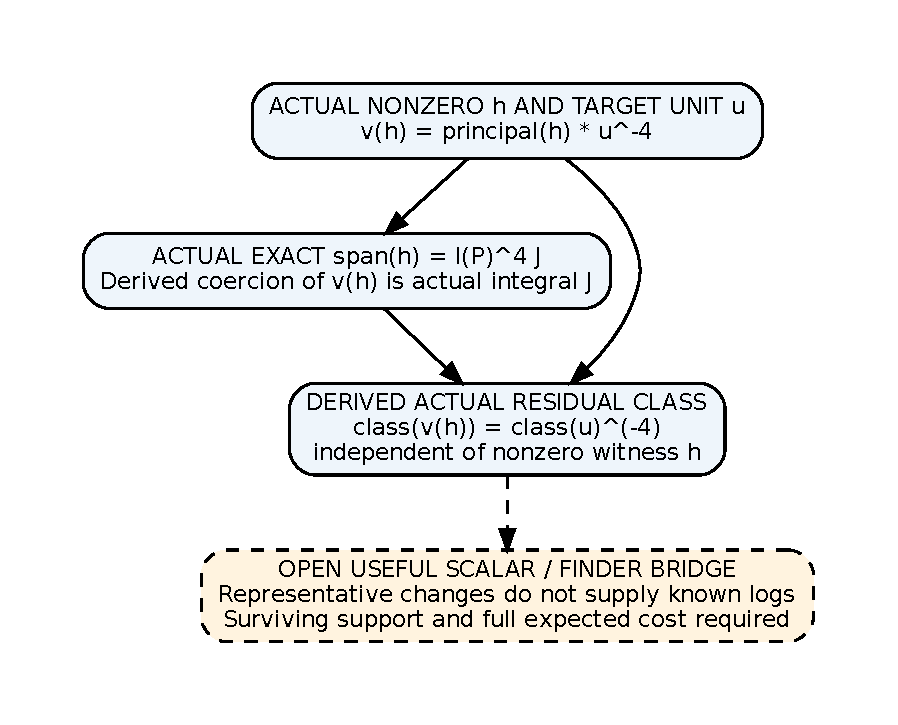
\includegraphics[height=2.4in,width=.97\linewidth,keepaspectratio]{residual-class-dependencies-001.pdf}\end{center}

\textbf{Derived maps.}
Injectivity of the actual coordinate-ring map into its function field makes
mapped \(h\) nonzero. The public principal-unit construction and its coercion
law identify its actual ideal. The target-unit power cancellation and exact
integral factorization identify the residual unit with \(J\). The public
principal-class criterion and class-group multiplication then give the class
formula and witness independence [pcc:unverified].

\textbf{Check and proof map.}
Source 080, build 086 and local receipt 042 check 205 local statements, five
new, exit zero, zero warnings, all printed foundations standard;267 direct
input bindings are checked. The five declarations are in the namespace below:
\begin{center}\begin{tabular}{l}
\texttt{OrientationActualResidualClass}\\
\texttt{principalUnit\_coe}, \texttt{residualUnit\_product}\\
\texttt{residualUnit\_coe}, \texttt{residualUnit\_class}\\
\texttt{residualUnit\_class\_independent}
\end{tabular}\end{center}
PCC-20261123-a97e80 is unsigned local data, outside historical shared
Transport53/57 audit/fresh [pcc:unverified].

\textbf{Sources, limitation and next test.}
Public Mathlib class-group principal-unit, principal-class and fractional-ideal
coercion laws are reused; no novelty claim is made for standard algebra.
Rejected079 unit-inverse projection mismatch and raw log remain exact;
accepted080 uses public \texttt{Units.inv\_mul} without a private-body override.
Witness variation can change the representative or splitting, but cannot change
this residual class. Neither a nonsplit field representation nor this class
formula supplies a discrete logarithm. Next test asymmetric branch conditions
and known point contributions that survive normalization, with actual kernel,
scalar-finder and full expected bit-cost obligations kept explicit.
\end{document}
